\ylDisplay{Sähvatus} % Ülesande nimi
{Mihkel Kree} % Autor
{lõppvoor} % Voor
{2006} % Aasta
{G 9} % Ülesande nr.
{10} % Raskustase
{
% Teema: Geomeetriline-optika
\ifStatement
Optiline süsteem koosneb kahest nõguspeeglist ja kumerläätsest (vt joonist), mille optilised peateljed ühtivad. Ringikujulise ristlõikega valgusimpulss siseneb süsteemi optilise peatelje sihis ning valgusvihu telg ühtib sellega. Peeglite kõverusraadiused on $R_1 = \SI{8}{m}$ ja $R_2 = \SI{4}{m}$ ning peeglite vahekaugus $L = \SI{6}{m}$. Peeglite läbimõõdud on $d_1 = \SI{160}{mm}$ ja $d_2 = \SI{96}{mm}$. Kiire läbimõõt on $D = \SI{192}{mm}$. Läätse läbimõõt on suurem valgusvihu omast. Suurema peegli keskel on ava läbimõõduga $d_0 = \SI{1}{mm}$. Joonistage valguse intensiivsuse ajaline kulg kumerläätse fookuses $f$. Eeldage, et süsteemi saabuva impulsi kestvus $\tau \ll L/c$. Valguse kiirus $c = \SI{3e8}{m/s}$.

\begin{center}
	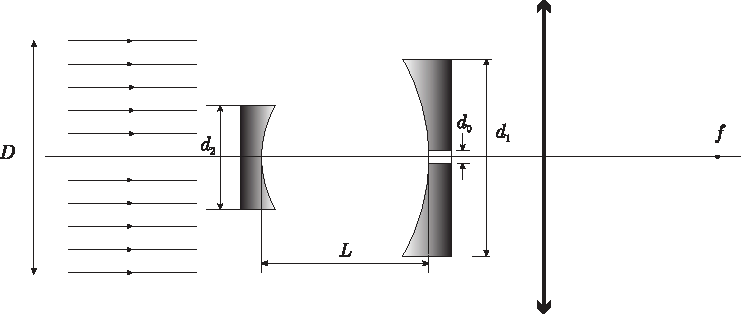
\includegraphics[width=0.95\linewidth]{2006-v3g-09-yl}
\end{center}
\fi


\ifHint
Ülesandes on arvandmed valitud nõnda, et peeglite fookused ühtiksid. Tõepoolest, nõguspeeglite fookuskaugus on pool raadiusest ja peeglite vahemaa on võrdne peeglite fookuskauguste summaga. See tähendab, et peale igat edasi-tagasi peegeldumist püsivad valguskimbu kiired paralleelselt, kusjuures kimp muutub 2 korda kitsamaks (sest fookuskauguste suhe on 2).
\fi


\ifSolution
Alustuseks paneme tähele suurepärast seost arvandmetes. Nimelt ühtivad peeglite fookused, sest peeglite vahemaa on võrdne peeglite fookuskauguste summaga. Nõguspeegli fookuskaugus on teatavasti pool raadiusest. Paralleelne kiirtekimp koondub peegli fookuses. Seepärast jääb paralleelne kiirtekimp antud süsteemis pärast kahekordset peegeldumist ikkagi paralleelseks. Kuid paneme tähele, et kiire laius väheneb kaks korda, sest ühe läätse fookuskaugus on kaks korda suurem teise omast.

Valguskiir jääb niisiis peeglite vahele pendeldama seniks, kuni tema kaugus teljest on väiksem kui $d_0/2 = \SI{0.5}{mm}$, kusjuures esialgne kauguste vahemiks, mis jõuab peegliteni on $d_2/2 = \SI{48}{mm}$ kuni $d_1/2 = \SI{80}{mm}$, ehk pilu läbimiseks peab valgusvihk koonduma $d_2/d_0 = 96$ kuni $d_1/d_0 = 160$ korda. Pärast $n$-kordset edasi-tagasi peegeldumist väheneb kiire kaugus teljest $2^n$ korda. Paneme tähele, et 128 on kahe aste ($2^7 = 128$). Seepärast väljub peeglile langenud kiir pilust kahes järgus: esimene osa pärast seitsmendat edasi-tagasi liikumist ning teine osa pärast kaheksandat. Üks edasi-tagasi liikumine peeglite vahel tekitab ajalise viivise $2L/c$.

Kumerläätsele langev paralleelne kiirtekimp koondub fookuses, kusjuures fookuseni jõudmise aeg ei sõltu kiire asukohast (teljelähedased kiired läbivad paksema klaasikihi kui kaugemad kiired, klaasi läbib valgus aga aeglasemalt). Niisiis on fookuses oodata kolme impulssi: peegli ümbert tulnud osa, pärast seitset edasi-tagasi peegeldumist tulnud osa ning pärast kaheksat. Nende impulsside ajaline vahe on vastavalt $14L/c$ ja $2L/c$.

Nüüd tuleb veel leida impulsside suhtelised intensiivsused, mis on võrdsed vastavate rõngaste pindaladega esialgse kiire ristlõikes. Esimese peegli läbimõõdust väiksem osa ei läbigi süsteemi. Kõige välimise rõnga pindala on võrdeline arvuga $192^2 - 160^2$, järgmisele impulsile vastav rõnga pindala $128^2 - 96^2$ ning viimasele impulsile vastava rõnga korral $160^2 - 128^2$. Need arvud suhtuvad kui: $32^2(6^2 - 5^2) : 32^2 (4^2 - 3^2) : 32^2 (5^2 - 4^2) = 11 : 7 : 9$.

\begin{center}
	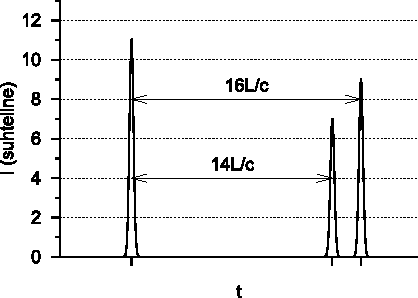
\includegraphics[width=0.6\linewidth]{2006-v3g-09-lah}
\end{center}
\fi
}